\documentclass[12pt]{article}

% layout
\usepackage[margin=1in]{geometry}
\usepackage{fancyhdr}
	\pagestyle{fancy}
	\setlength{\headheight}{16pt} % correct for headheight error
	% title
	\lhead{MP0}
	\chead{ECE549}
	\rhead{Yen-Ting Liu}

% images
\usepackage{graphicx}
	\graphicspath{{images/}}

% typeset
\usepackage{titlesec}
	% make section title comply with homework template
	\titleformat
		{\section}
		{\normalfont\large\bfseries}{Part \thesection: }
		{0em}{}
\usepackage{enumitem}
	\setlist[enumerate]{align=left}

% pretty table
\usepackage{booktabs}

% math symbols
\usepackage[fleqn]{amsmath}
\usepackage{mathtools} % provide dcases, will also load amsmath
\usepackage{amssymb}
\usepackage{esint}
	% make eqref compatible with hyperref
	\makeatletter
	\renewcommand*{\eqref}[1]{%
		\hyperref[{#1}]{\textup{\tagform@{\ref*{#1}}}}%
	}
	\makeatother
\usepackage{ulem}

% equations
\usepackage{nicefrac}
\usepackage{cases}
\usepackage[makeroom]{cancel} % crossed-out

% code highlights
\usepackage{xcolor}
\usepackage{listings}
	\lstset{
		basicstyle=\footnotesize\ttfamily,
		keywordstyle=[1]\ttfamily\color{blue}\bfseries,
		identifierstyle=\ttfamily\color{purple}\bfseries,
		commentstyle=\normalfont\color{green},
		stringstyle=\color{brown}\ttfamily,
		columns=fullflexible,
		fontadjust=true,
	}

% reference
\usepackage{hyperref}
\usepackage[noabbrev]{cleveref}

\begin{document}

\section{Linear Interpolation}
	% 1) insert your linear interpolated test image (hope.jpg)
	The reconstructed test image (\lstinline{hope.jpg}) is shown as \cref{fig:hope-recon-linear}.
	\begin{figure}[h]
		\centering
		\caption{Test image reconstructed by linear interpolation.}
		\label{fig:hope-recon-linear}
		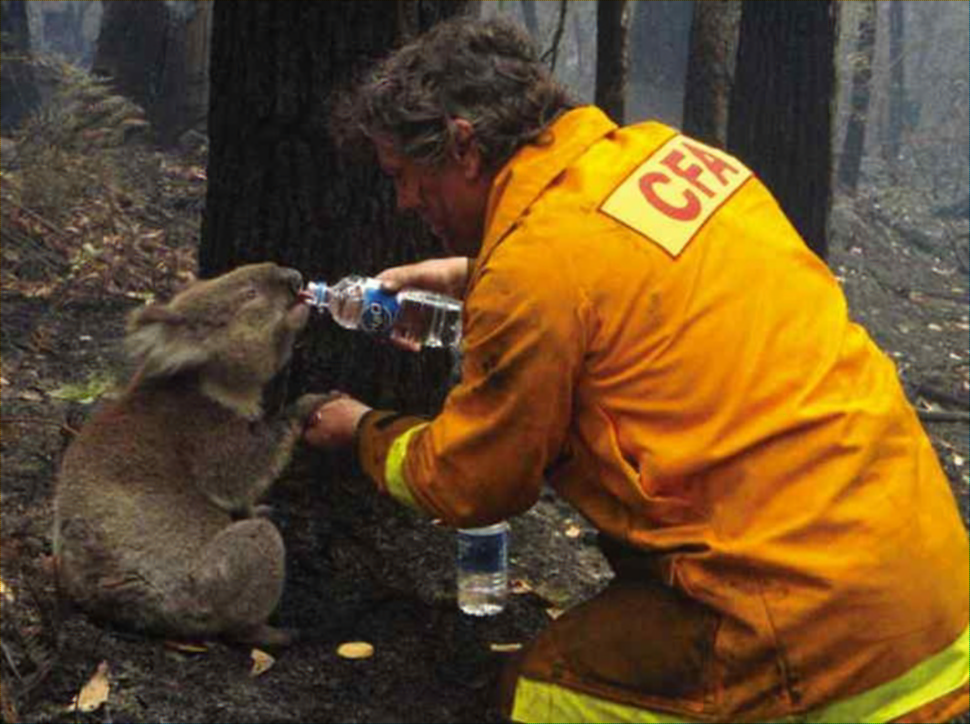
\includegraphics[width=8cm]{hope_recon_lin.png}
	\end{figure}

	% 2) display the map of all 3 training images here
	% 3) close up of any artifacts you came across
	% 4) average_per_pixel error and max_pixel_error for each of 3 training
	The template asked for \textit{map of squared differences}, I interpreted this as mean squared error (MSE):
	\begin{equation*}
		\text{MSE} = \frac{1}{N} \sum_{i,j} (Y_{ij}^c - \hat{Y}_{ij}^c)^2
	\end{equation*}
	where $Y_{ij}^c$ is the reconstructed pixel value of color $c$, $\hat{Y}$ denotes the original image, and $N$ is the total number of pixels.
	MSE and maximum pixel error is listed in \cref{tab:errors-linear}.

	\begin{table}[h]
		\centering
		\caption{Errors of provided images.}
		\label{tab:errors-linear}
		\begin{tabular}{c|cc}
			\toprule
			Image & MSE & max pixel error \\
			\midrule
			Crayons & & \\
			Tony & & \\
			Iceberg & & \\
			\bottomrule
		\end{tabular}
	\end{table}

\section{Freeman Method}
	Next section.

\section{Images of my choice}
	Some image choices.

\section{Bonus}
	Bonus!

\end{document}